\section{Orthogonal Basis States}

\frame{
    \frametitle{Initial Attempt at a Basis Set}
    \begin{columns}
        \begin{column}{0.4\textwidth}
            \begin{center} 
            Basis Set
            \resizebox{0.4\textheight}{!}{\begin{tabular}{ |l|l|l| }
                \hline
                \textbf {$\kappa_{2V}$} & \textbf {$\kappa_\lambda$} & \textbf {$\kappa_V$} \\
                \hline
                1   &  1 &   1 \\
                1   &  0 &  -1 \\
                0   &  1 &   1 \\
                1.5 &  1 &   1 \\
                1   &  2 &   1 \\
                2   &  1 &  -1 \\
                \hline
            \end{tabular}} \end{center}
        \end{column}
        \begin{column}{0.6\textwidth}
            Linear Combination Equation
            \vspace{10mm}

            {\tiny $
A_{0} \left(- 2 \kappa_{2V}^{2} + 6 \kappa_{2V} \kappa_{V}^{2} - 3 \kappa_{2V} \kappa_{V} \kappa_{\lambda} - 4 \kappa_{V}^{4} + 5 \kappa_{V}^{3} \kappa_{\lambda} - \kappa_{V}^{2} \kappa_{\lambda}^{2}\right) + A_{1} \left(- \frac{3 \kappa_{2V} \kappa_{V}^{2}}{2} + \frac{3 \kappa_{2V} \kappa_{V} \kappa_{\lambda}}{2} + \frac{5 \kappa_{V}^{4}}{2} - 3 \kappa_{V}^{3} \kappa_{\lambda} + \frac{\kappa_{V}^{2} \kappa_{\lambda}^{2}}{2}\right) + A_{2} \left(\frac{2 \kappa_{2V}^{2}}{3} - \frac{11 \kappa_{2V} \kappa_{V}^{2}}{6} + \frac{\kappa_{2V} \kappa_{V} \kappa_{\lambda}}{6} + \frac{7 \kappa_{V}^{4}}{6} - \frac{\kappa_{V}^{3} \kappa_{\lambda}}{6}\right) + A_{3} \left(\frac{4 \kappa_{2V}^{2}}{3} - \frac{8 \kappa_{2V} \kappa_{V}^{2}}{3} + \frac{4 \kappa_{2V} \kappa_{V} \kappa_{\lambda}}{3} + \frac{4 \kappa_{V}^{4}}{3} - \frac{4 \kappa_{V}^{3} \kappa_{\lambda}}{3}\right) + A_{4} \left(- \frac{\kappa_{2V} \kappa_{V}^{2}}{2} + \frac{\kappa_{2V} \kappa_{V} \kappa_{\lambda}}{2} + \frac{\kappa_{V}^{4}}{2} - \kappa_{V}^{3} \kappa_{\lambda} + \frac{\kappa_{V}^{2} \kappa_{\lambda}^{2}}{2}\right) + A_{5} \left(\frac{\kappa_{2V} \kappa_{V}^{2}}{2} - \frac{\kappa_{2V} \kappa_{V} \kappa_{\lambda}}{2} - \frac{\kappa_{V}^{4}}{2} + \frac{\kappa_{V}^{3} \kappa_{\lambda}}{2}\right)
$
}
        \end{column}
    \end{columns}
}

\displaythree{Comparing Linear Combination with Generated Sample}{
    {\tiny The linear combination successfully fits separately generated MC samples}
}{mHH_cvv0p5cl1p0cv1p0}
{mHH_cvv2p0cl1p0cv1p0}
{mHH_cvv0p0cl0p0cv1p0}

\displaythree{More plots}{
    {\small The $\kappa_{2V}=1, \kappa_\lambda=10, \kappa_V=1$ state shows large discrepencies, indicating room for improvement.}

    \vspace{5mm}


    { \tiny Note that the basis $\kappa_{2V}=1,\kappa_\lambda=0,\kappa_V=-1$ is one of the basis states. }

}{mHH_cvv0p0cl0p0cv1p0}
{mHH_cvv1p0cl0p0cv-1p0}
{mHH_cvv1p0cl10p0cv1p0}


\fullscreenimage{Looking at Many Bases at Once}{coupling_scan_rnd_base}
\fullscreenimage{Normalize each distribution to its own integral}{coupling_scan_rnd_hori}
\fullscreenimage{Log Helps, but 'best' states are still unclear}{coupling_scan_rnd_hori_log}
\fullscreenimage{Normalizing to max-per-bin highlights where states excel}{coupling_scan_rnd_hash_max}



\frame{
    \frametitle{Optimal Basis States for New Production }
    \begin{columns}
        \begin{column}{0.33\textwidth}
            \begin{center} 
            \resizebox{0.3\textheight}{!}{\begin{tabular}{ |l|l|l| }
                \hline
                \textbf {$\kappa_{2V}$} & \textbf {$\kappa_\lambda$} & \textbf {$\kappa_V$} \\
                \hline
                 1.  &  1. &  1.  \\
                 1.5 &  1. &  1.  \\
                 2.  &  1. &  1.  \\
                 1.  &  0. &  1.  \\
                 1.  & 10. &  1.  \\
                 1.  &  1. &  0.5 \\
                \hline
            \end{tabular}}

            \begin{figure}
                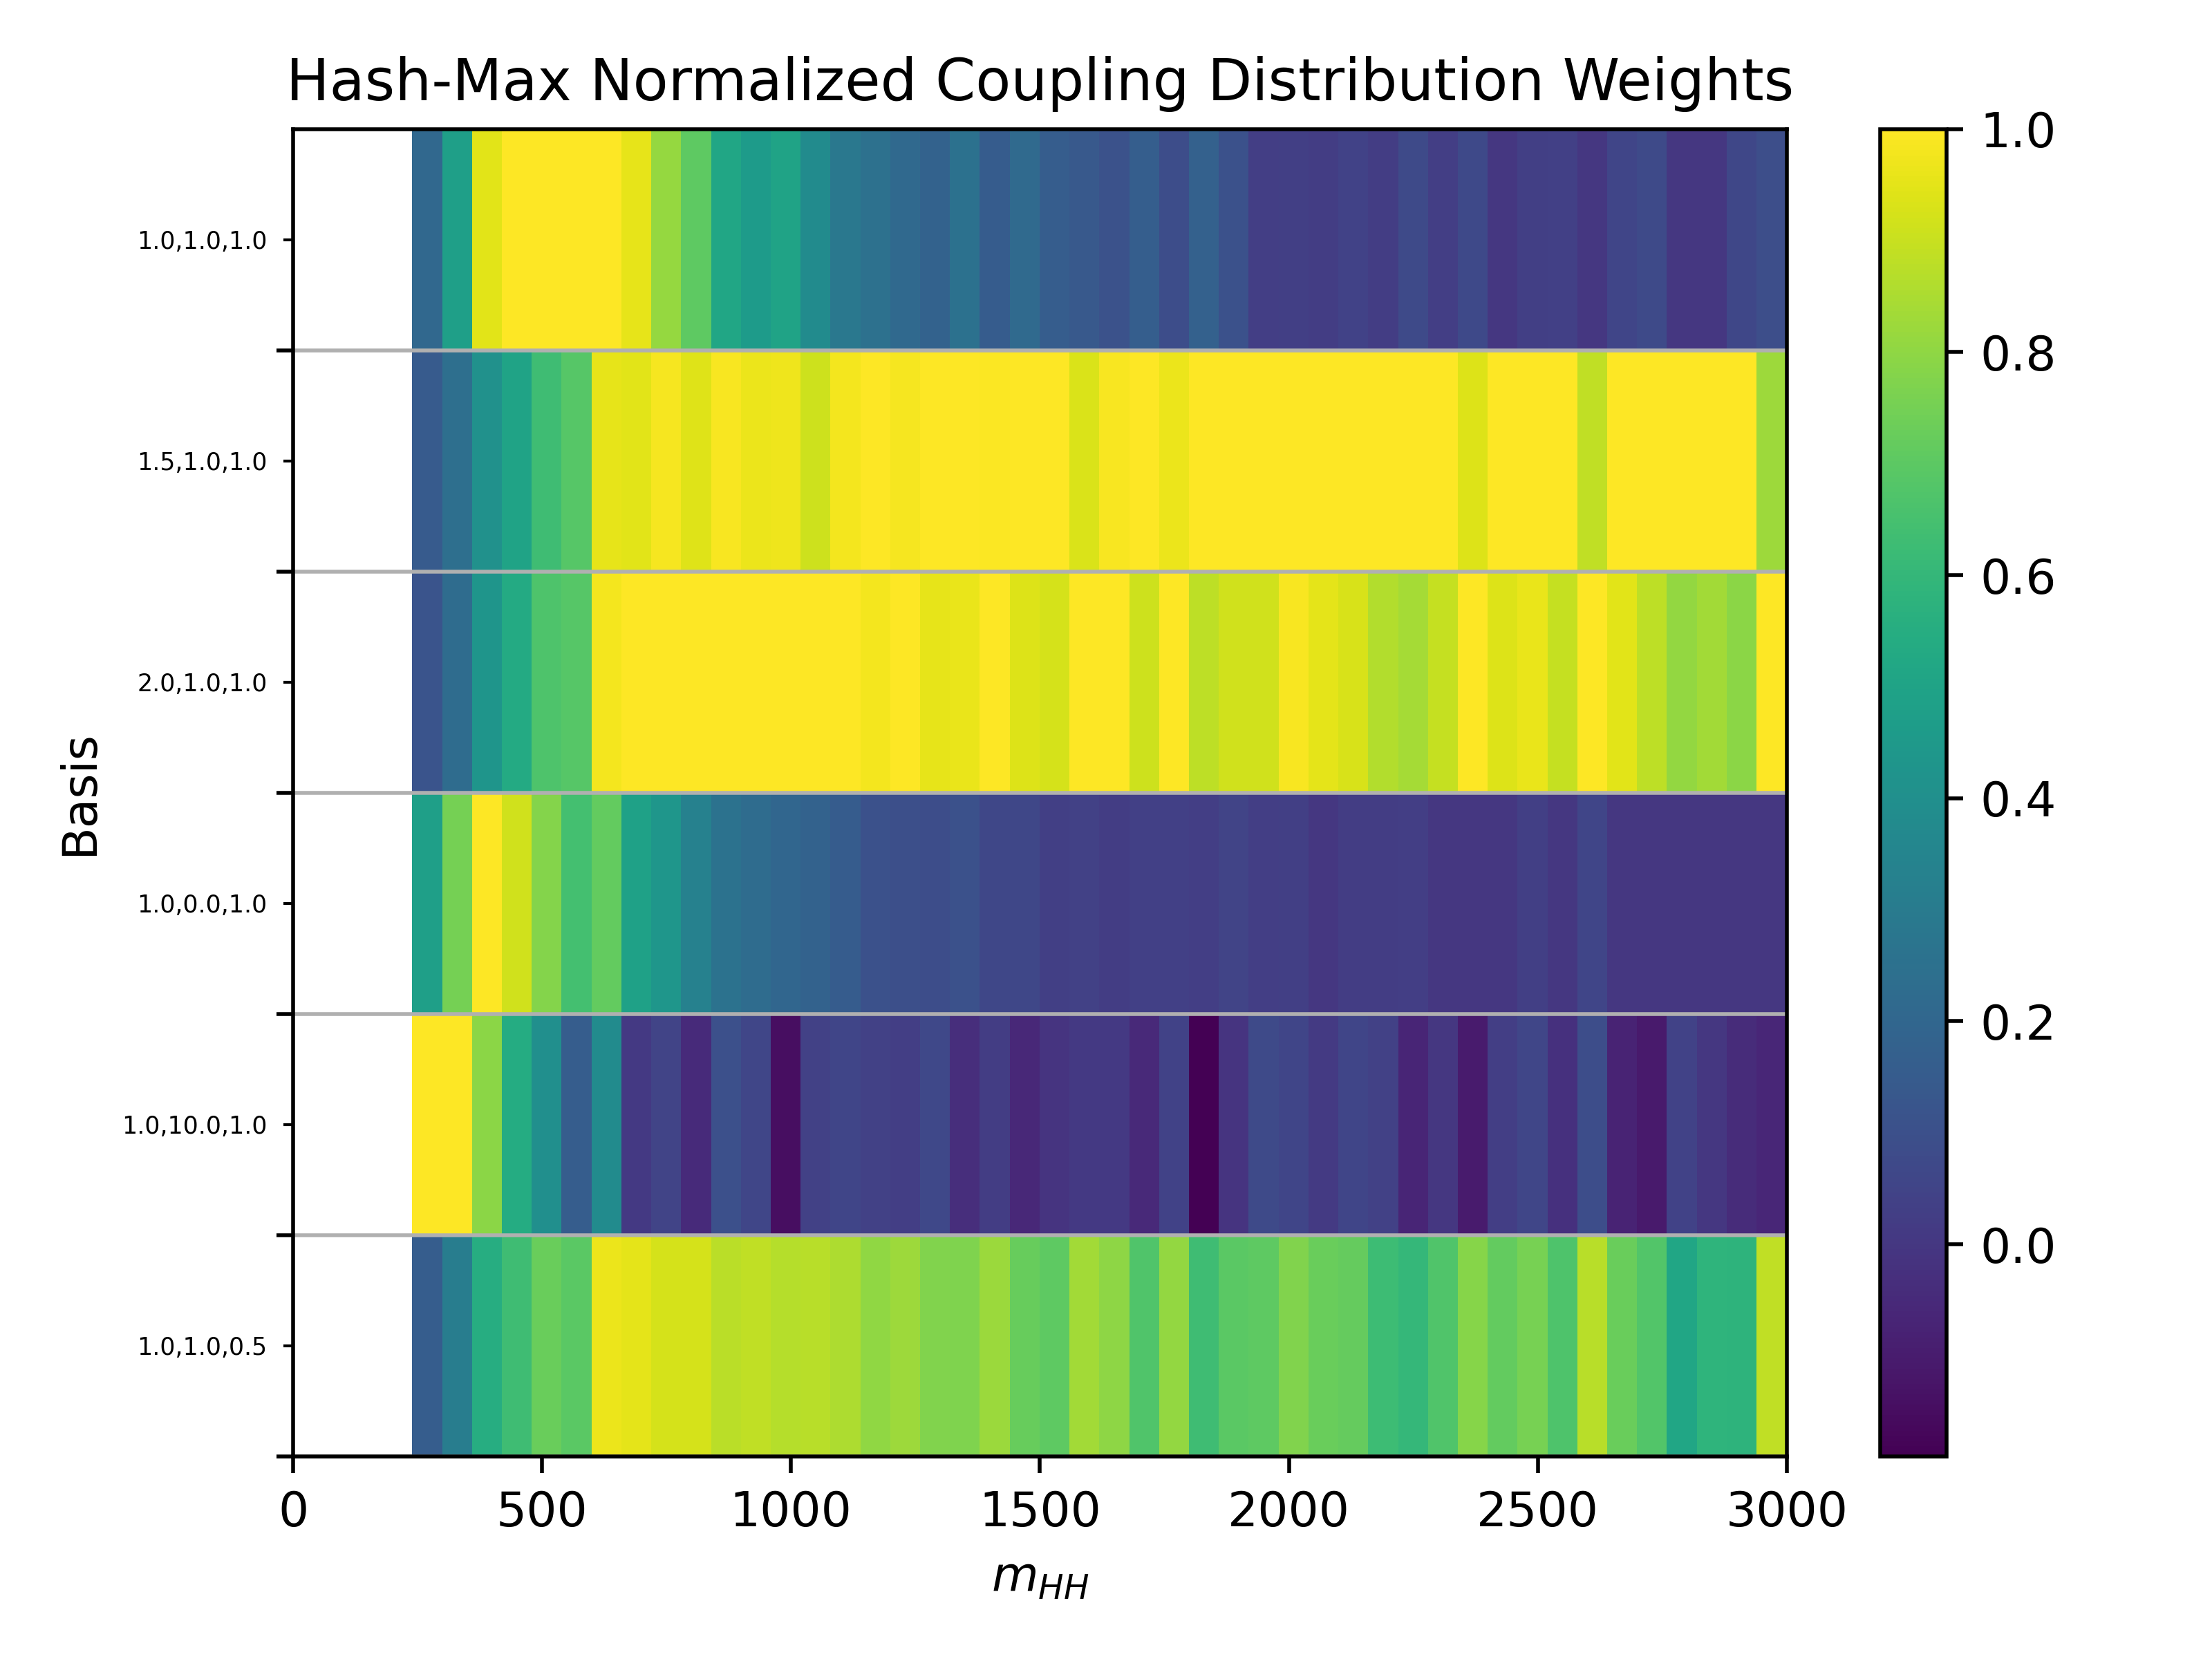
\includegraphics[width=\linewidth,height=\textheight,keepaspectratio]
                {coupling_scan_auto_chosenR0_hash_max}
            \end{figure}

            \end{center}
        \end{column}
        \begin{column}{0.33\textwidth}
            \begin{center} 
            \resizebox{0.3\textheight}{!}{\begin{tabular}{ |l|l|l| }
                \hline
                \textbf {$\kappa_{2V}$} & \textbf {$\kappa_\lambda$} & \textbf {$\kappa_V$} \\
                \hline
                 1.  &  1. &  1.  \\
                 1.5 &  1. &  1.  \\
                 2.  &  1. &  1.  \\
                 1.  &  0. &  1.  \\
                 1.  & 10. &  1.  \\
                 1.  &  1. &  1.5 \\
                \hline
            \end{tabular}}

            \begin{figure}
                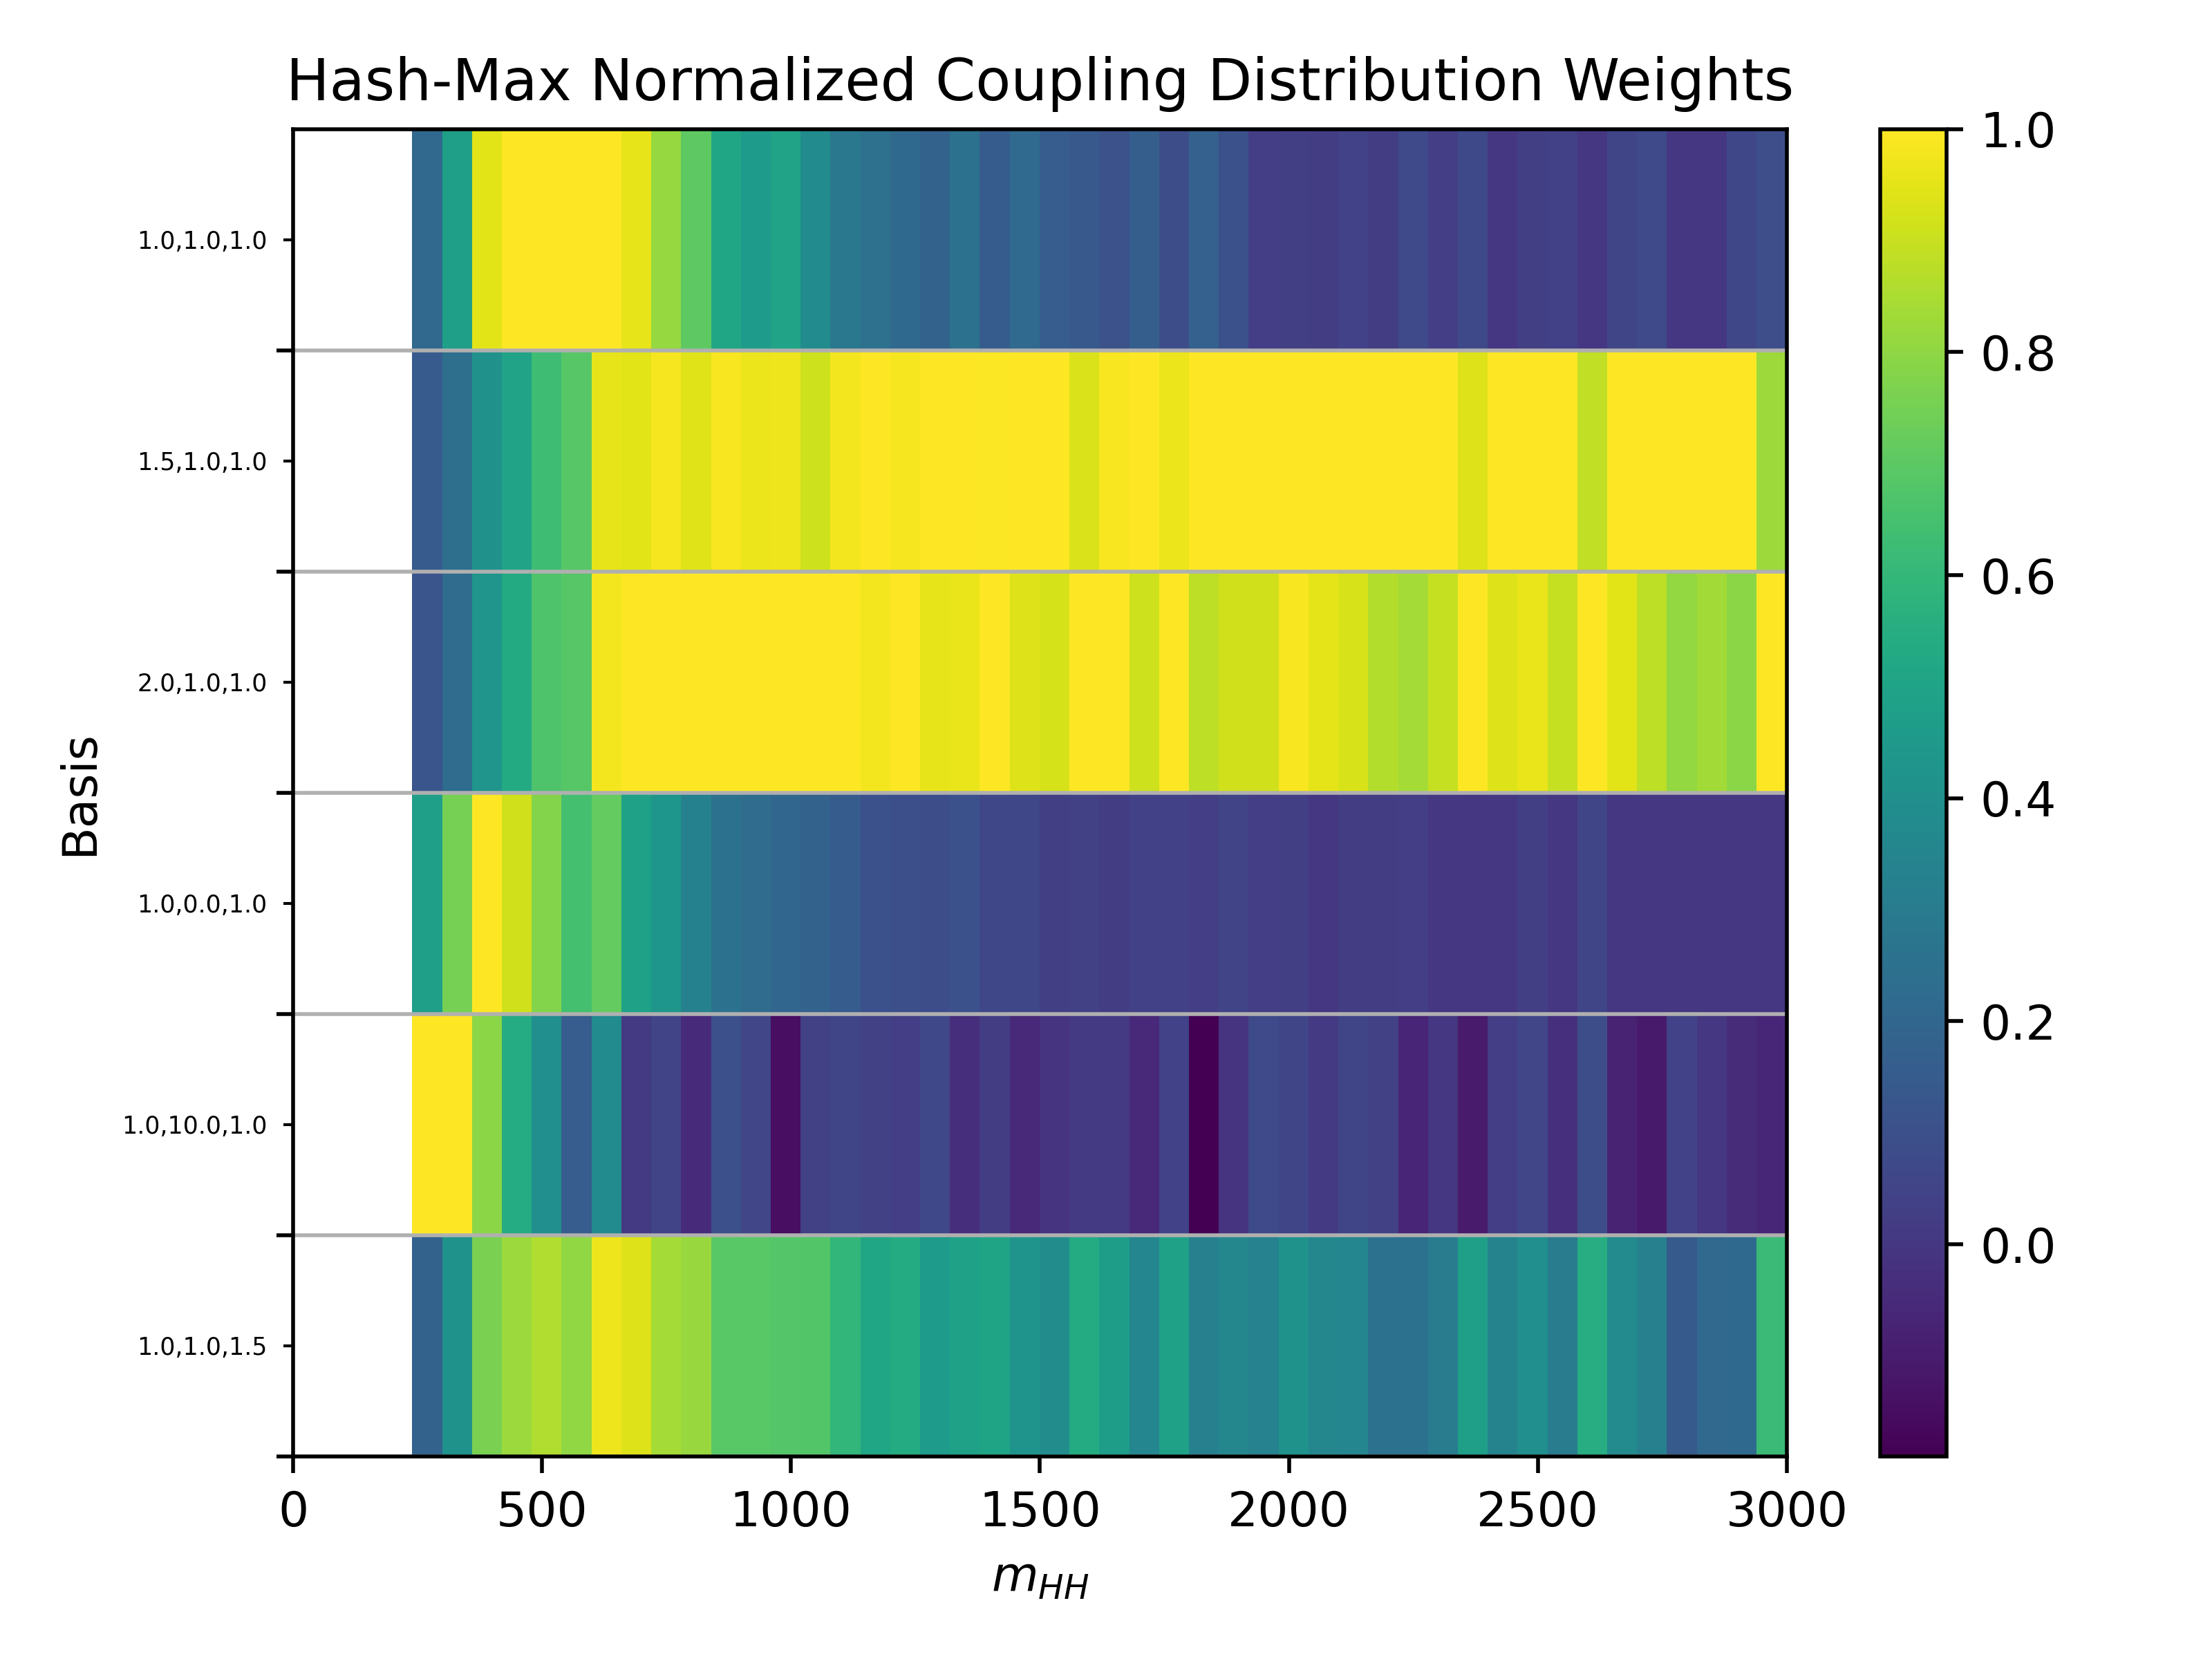
\includegraphics[width=\linewidth,height=\textheight,keepaspectratio]
                {coupling_scan_auto_chosenR1_hash_max}
            \end{figure}

            \end{center}
        \end{column}
        \begin{column}{0.33\textwidth}
            \begin{center} 
            \resizebox{0.3\textheight}{!}{\begin{tabular}{ |l|l|l| }
                \hline
                \textbf {$\kappa_{2V}$} & \textbf {$\kappa_\lambda$} & \textbf {$\kappa_V$} \\
                \hline
                 1.  &  1. &  1.  \\
                 1.5 &  1. &  1.  \\
                 2.  &  1. &  1.  \\
                 1.  &  0. &  1.  \\
                 1.  & 10. &  1.  \\
                 0.  &  0. &  1.  \\
                \hline
            \end{tabular}}

            \begin{figure}
                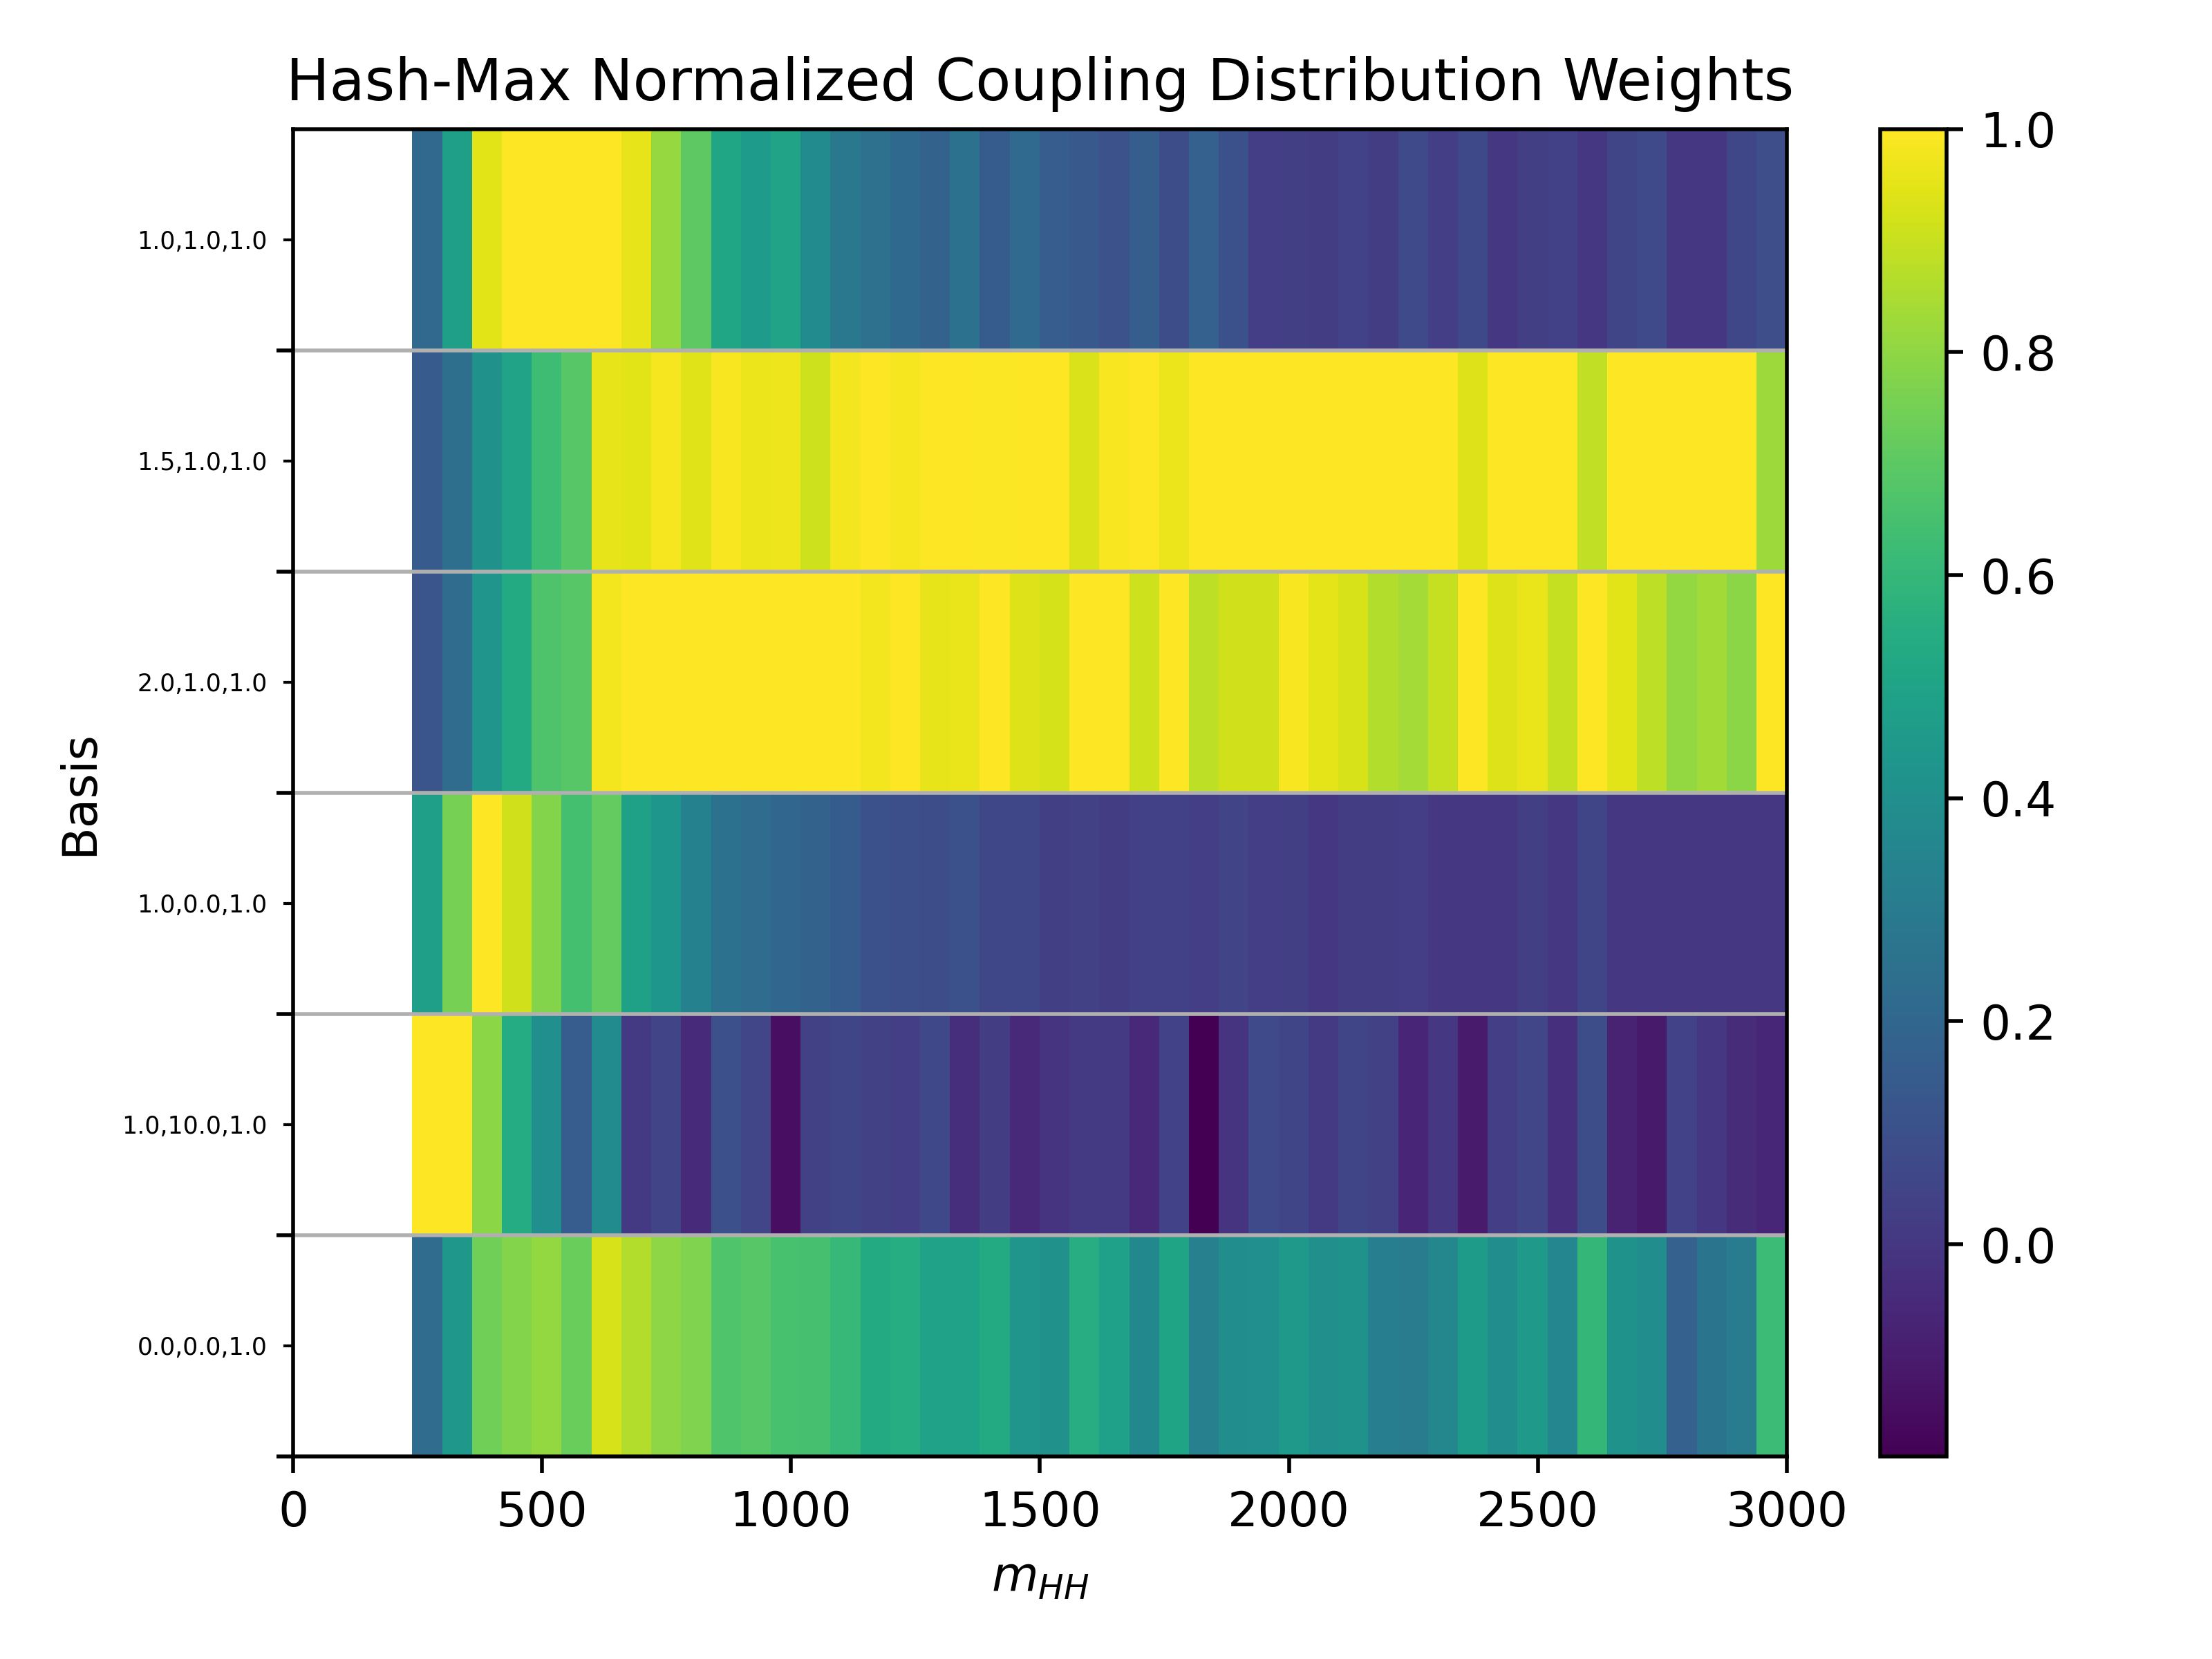
\includegraphics[width=\linewidth,height=\textheight,keepaspectratio]
                {coupling_scan_auto_chosenR2_hash_max}
            \end{figure}

            \end{center}
        \end{column}
    \end{columns}
}
